\chapter{Phonemized CHILDES: A Phonemic Multi-Lingual Corpus of Child-Directed Speech}

\begin{roughdraft}
    The first content chapter of the thesis. Motivated by the need to have good quality multi-lingual phonemic datasets to do child acquisition experiments, it covers the following:
    \begin{itemize}[label=--]
        \item Motivation for using automated transcription tools to create phonemic datasets for language modeling (possibly covered in introduction). Movitation for having one multi-lingual dataset with a unified IPA format.
        \item Specific background related to datasets that exist (possibly covered in background chapter) and transcription tools that exist. Discuss the challenges behind creating phonemized datasets, the issues with IPA and previous approaches.
        \item Description of the Corpus Phonemizer tool, how it works and what it can do.
        \item The use of Corpus Phonemizer to produce Phonemized CHILDES. Describe Phonemized CHILDES dataset and what choices were made. 
        \item Corpus Analysis of Phonemized CHILDES across a wide range of experiments. 
    \end{itemize}
\end{roughdraft}

\section{Introduction and Background}
\label{sec:dataset-intro}

\rough{Specific background related to datasets that exist (possibly covered in background chapter) and transcription tools that exist. Discuss the challenges behind creating phonemized datasets, the issues with IPA and previous approaches.}

\section{Corpus Phonemizer}
\label{sec:dataset-corpus-phonemizer}

\rough{Description of the Corpus Phonemizer tool, how it works and what it can do. In this intro, present what we want the output to be, how phonemes are separated by boundary markers etc.}



\subsection{Transcription tool backends}

\rough{Describe phonemizer, epitran, pinyintoipa, pingyam}

\subsection{Phoneme inventory validation}

\rough{Describe process of "folding". Introduce Phoible database and describe process used to create folding dictionaries for each language (maybe with a flow chart or algorithm). Say that I end up making folding dictionaries for the backend-language pairs used for Phonemized CHILDES.}

\subsection{Usage and Limitations}

\rough{Describe overall usage of tool and how it can be used. Call forward to next section where it is used to produce the Phonemized CHILDES dataset. Briefly mention how it also used to create Phonemized BabyLM datset and can be used for evaluation data as well, calling forward to next chapter. Discuss limitations of the tool. }

\section{Phonemized CHILDES}
\label{sec:dataset-corpus-phonemizer}

\rough{The use of Corpus Phonemizer to produce Phonemized CHILDES. Describe CHILDES, what languages are available, how the data is phonemized. Describe resulting dataset. In this intro, describe how all this code is saved as part of the Corpus Phonemizer suite as a tool called CHILDES processor.}

\begin{figure}
    \centering
    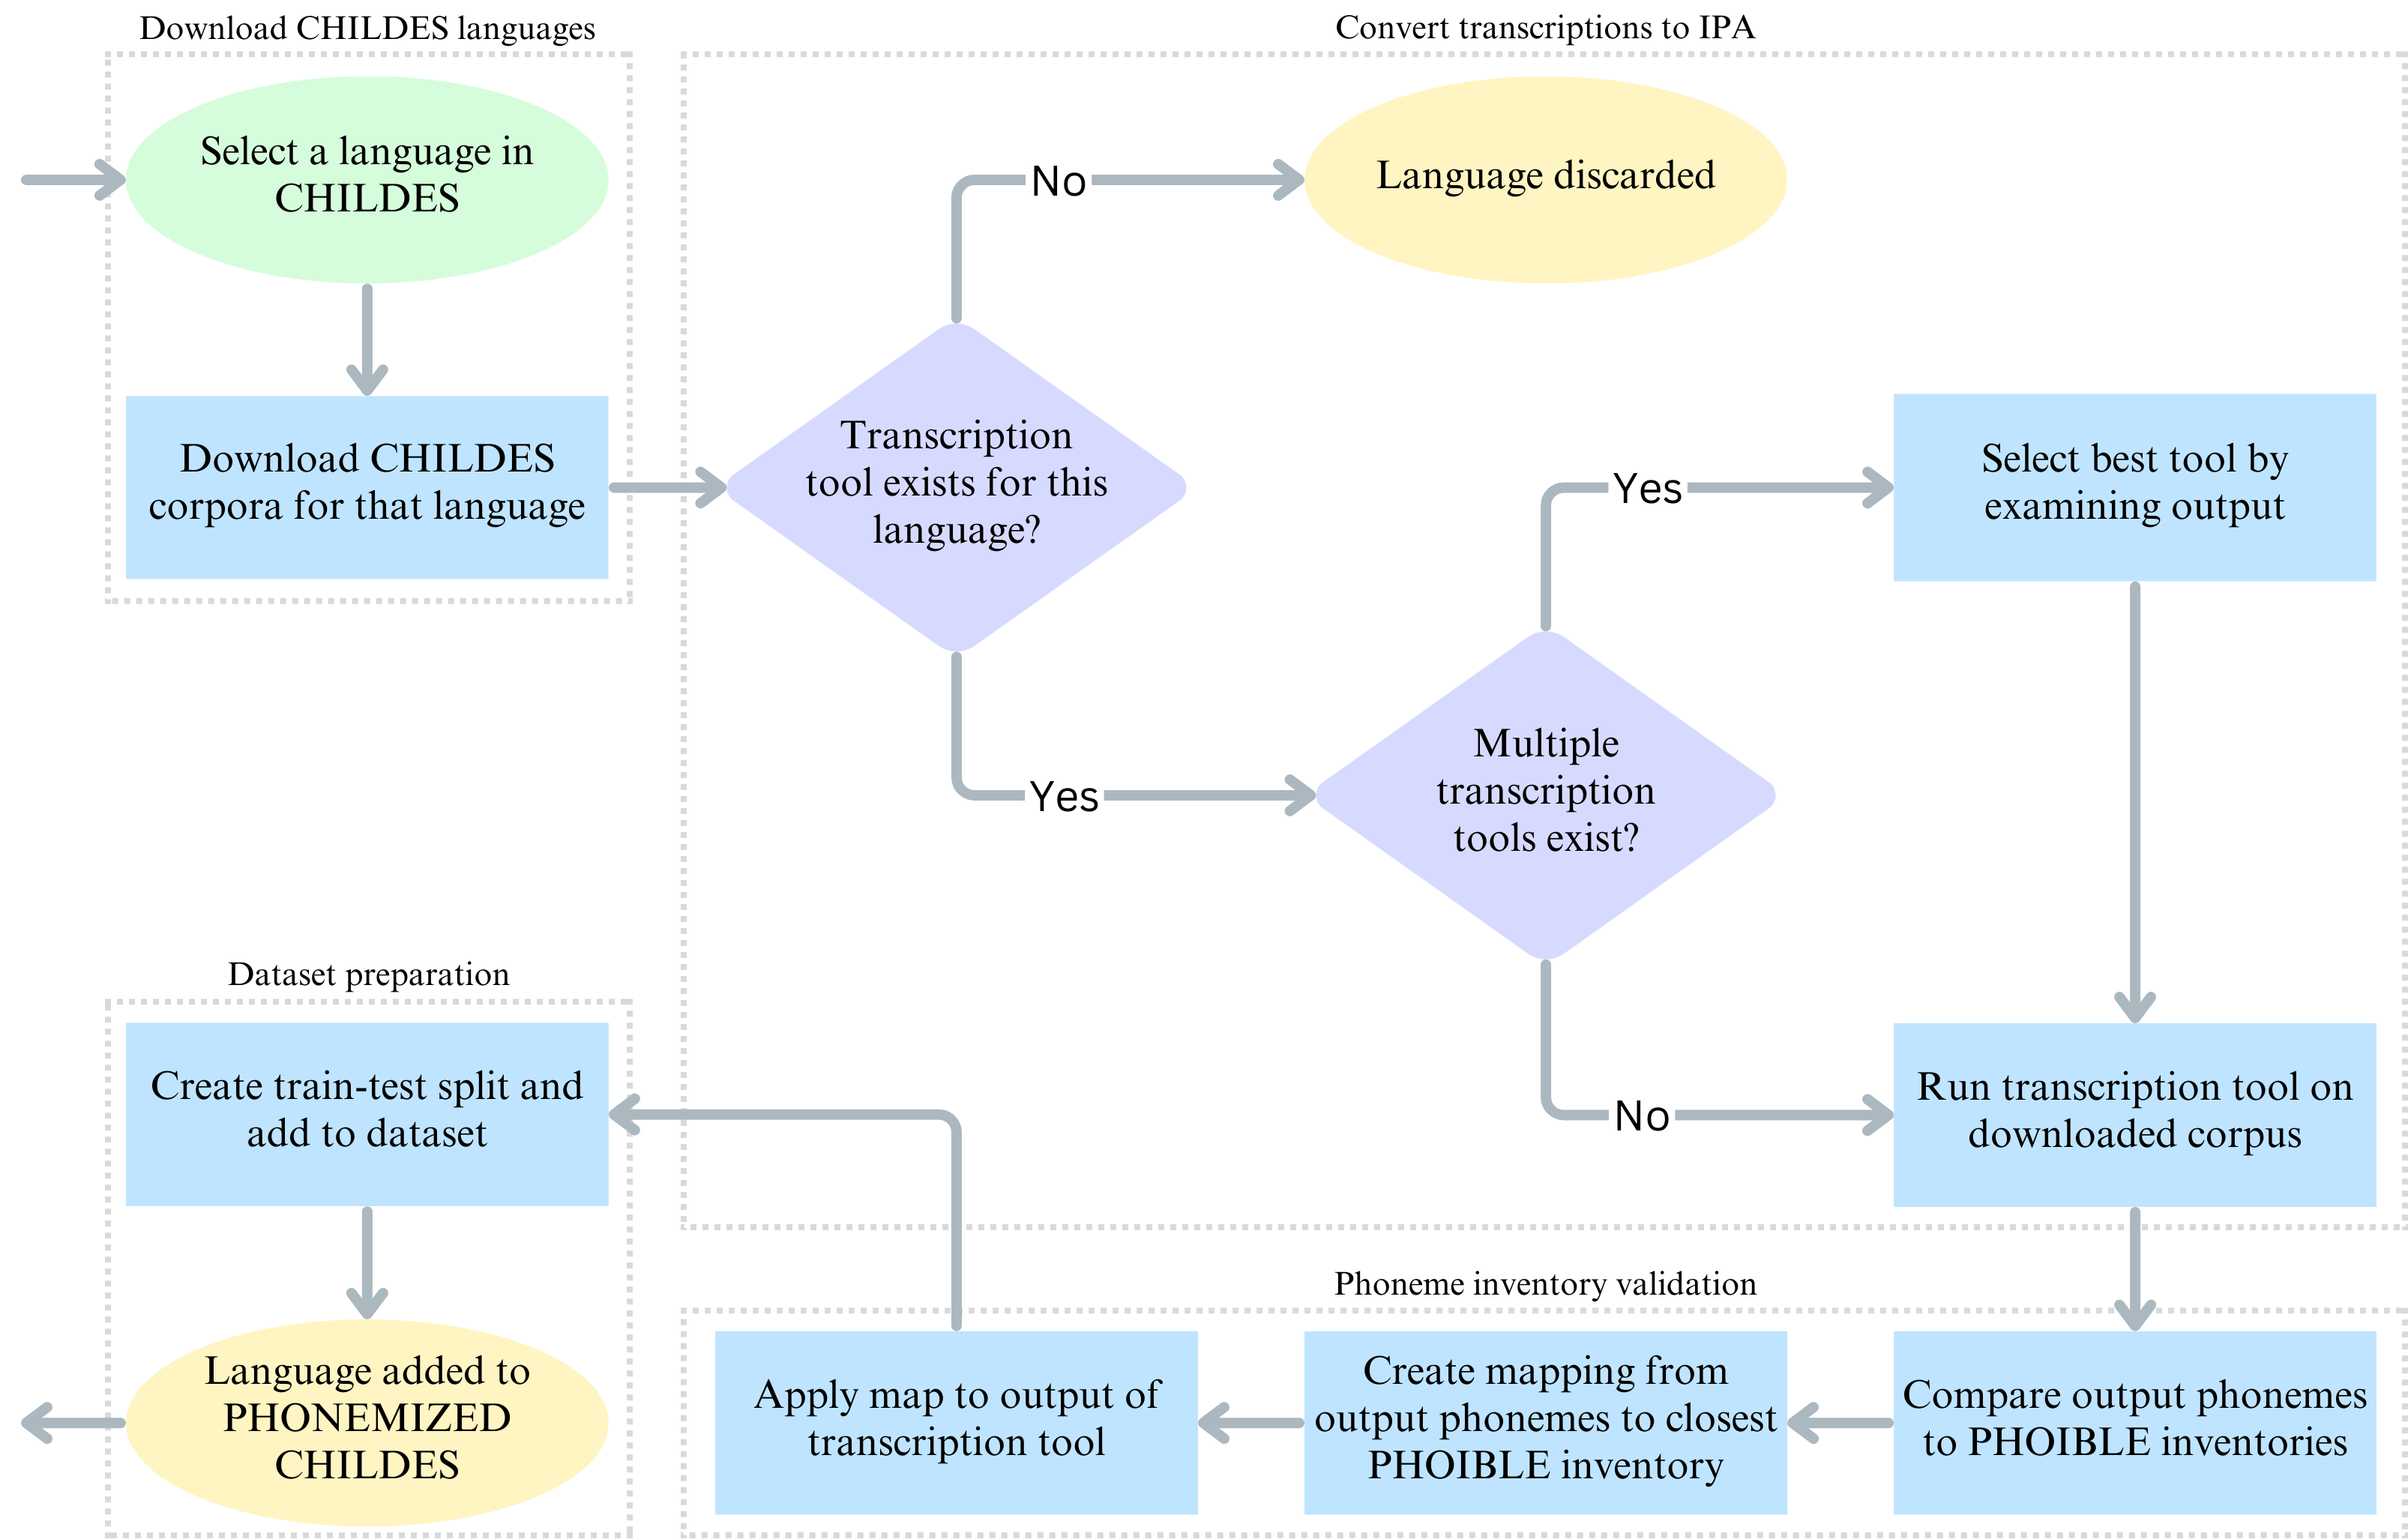
\includegraphics[width=0.9\linewidth]{Figures/13Dataset/data-prep.png}
    \caption{Data preparation pipeline for the Phonemized CHILDES dataset.}
    \label{fig:dataset-data-prep}
\end{figure}

\subsection{CHILDES}

\rough{Describe CHILDES and what languages are in there. Describe what data is available and how we download it.}

\subsection{Dataset creation}

\rough{I add a tool called CHILDES processor to the Corpus Phonemizer suite to specifically help with downloading, phonemizing, and preparing CHILDES corpora into a huggingface dataset. Given the range of languages in CHILDES, I need to determine which backend to use for each. I then need to examine the output and try to map it to a standard inventory set for that language. Finally, I save each language as a section of a Huggingface dataset, each language is a section and has a train-test split.}

\subsection{Dataset overview}

\rough{Describe resulting dataset, give a large table with details, which tool was used, which inventory we map to, etc.}

\section{Corpus Analysis}

\rough{This is where I use the corpus to analyse the phonemic properties of languages. Experiments include:
\begin{itemize}
    \item Information theoretic properties (Zipf's law, Heap's law, ratios, information rate, n-gram perplexities)
    \item Comparing phoneme properties to character properties (hypothesis: information rate more consistent across langugages when looking at phonemes rather than characters)
    \item Child vs adult speech (extract child utterances in CHILDES and compare MLU, word length etc)
    \item Child-directed vs adult-directed speech (compare CHILDES to BNC)
    \item Phoneme clustering (could possibly be moved to chapter 5 - segmentation): looking at phoneme clusters, possibly vowel harmony and other signals for segmentation.
    \item Child errors (could be moved to chapter 6 - past tense formation): looking at errors that children produce.
\end{itemize}
}